\documentclass[11pt]{article}
\usepackage[margin=1in]{geometry}
\usepackage{graphicx}
\usepackage{booktabs}
\usepackage{amsmath}
\usepackage{hyperref}
\title{RK vs NN proton reconstruction on breakup g4output \\ \large Head-to-head evaluation}
\date{2026-06-18}
\begin{document}
\maketitle

\begin{abstract}
This report evaluates proton reconstruction quality on the d+Sn breakup sample (ypol + zpol, 176 cells) using two backends: RK (Runge-Kutta least-squares fitter, three-point-free mode, run on spana03) and NN (6-128-128-64 MLP, formal\_B115T3deg/20260420\_184345 model, run locally). Both reconstructions derive from the same Geant4 g4output, enabling per-event entry-index alignment. Three error sets are reported for protons (RK-vs-truth, NN-vs-truth, RK-vs-NN), plus truth-vs-reco residuals for neutrons (NEBULA $\beta$-method, identical for both backends). Sample: 3301419 truth-proton events total.
\end{abstract}

\section{Data \& method}
\textbf{RK reco}: spana03 \texttt{data/reconstruction/dbreak\_elastic/}, 176 files, produced 2026-05-09 via \texttt{run\_dbreak\_elastic\_pipeline.py stage\_reco} with \texttt{--backend rk --rk-fit-mode three-point-free --max-iterations 40}. \\
\textbf{NN reco}: local \texttt{data/reconstruction/breakup\_nn\_20260503/}, 176 files, produced 2026-05-03 via \texttt{01\_run\_nn\_reco.sh} with the clean production model \texttt{formal\_B115T3deg/20260420\_184345}. \\
\textbf{g4output source}: identical for both backends (verified by file size 285252607 bytes, timestamp 2026-05-01 20:16:46 +0900). Per-event entry-index alignment is valid 1:1. \\
\textbf{Frame convention}: target frame (beam-as-Z) throughout. Truth is already target-frame; both backends' reco is rotated to target frame at write time via \texttt{RotateRecoResultToTargetFrame} (\texttt{apps/run\_reconstruction/main.cc:629-630}). No additional rotation in this analysis. \\
\textbf{Multi-proton events}: pick candidate whose $|p|$ is closest to truth (matches \texttt{evaluate\_target\_momentum\_reco.cc:347-359}).

\section{Proton reconstruction --- RK vs NN vs truth}
\subsection{Global residuals}
\begin{table}[h]\centering\small\begin{tabular}{lllll}\toprule
Pol & Backend & $\Delta p_x$ & $\Delta p_y$ & $\Delta p_z$ \\\midrule
ypol & RK & MAE=11.4, RMSE=39.7, Bias=-6.8, P95=30.7, N=2150443 & MAE=1.6, RMSE=3.5, Bias=-0.1, P95=4.1, N=2150443 & MAE=20.3, RMSE=87.8, Bias=-11.1, P95=26.8, N=2150443 \\
ypol & NN & MAE=6.1, RMSE=13.3, Bias=-1.8, P95=14.4, N=2150443 & MAE=1.3, RMSE=2.4, Bias=+0.5, P95=3.2, N=2150443 & MAE=6.6, RMSE=15.7, Bias=+2.8, P95=15.2, N=2150443 \\
zpol & RK & MAE=12.0, RMSE=46.8, Bias=-7.4, P95=35.3, N=101662 & MAE=1.7, RMSE=4.8, Bias=-0.2, P95=3.9, N=101662 & MAE=21.2, RMSE=91.8, Bias=-11.3, P95=30.8, N=101662 \\
zpol & NN & MAE=7.1, RMSE=13.7, Bias=-2.6, P95=22.2, N=101662 & MAE=1.4, RMSE=3.0, Bias=+0.6, P95=3.3, N=101662 & MAE=7.6, RMSE=15.5, Bias=+3.4, P95=23.8, N=101662 \\
\bottomrule\end{tabular}\end{table}
\begin{figure}[h]\centering
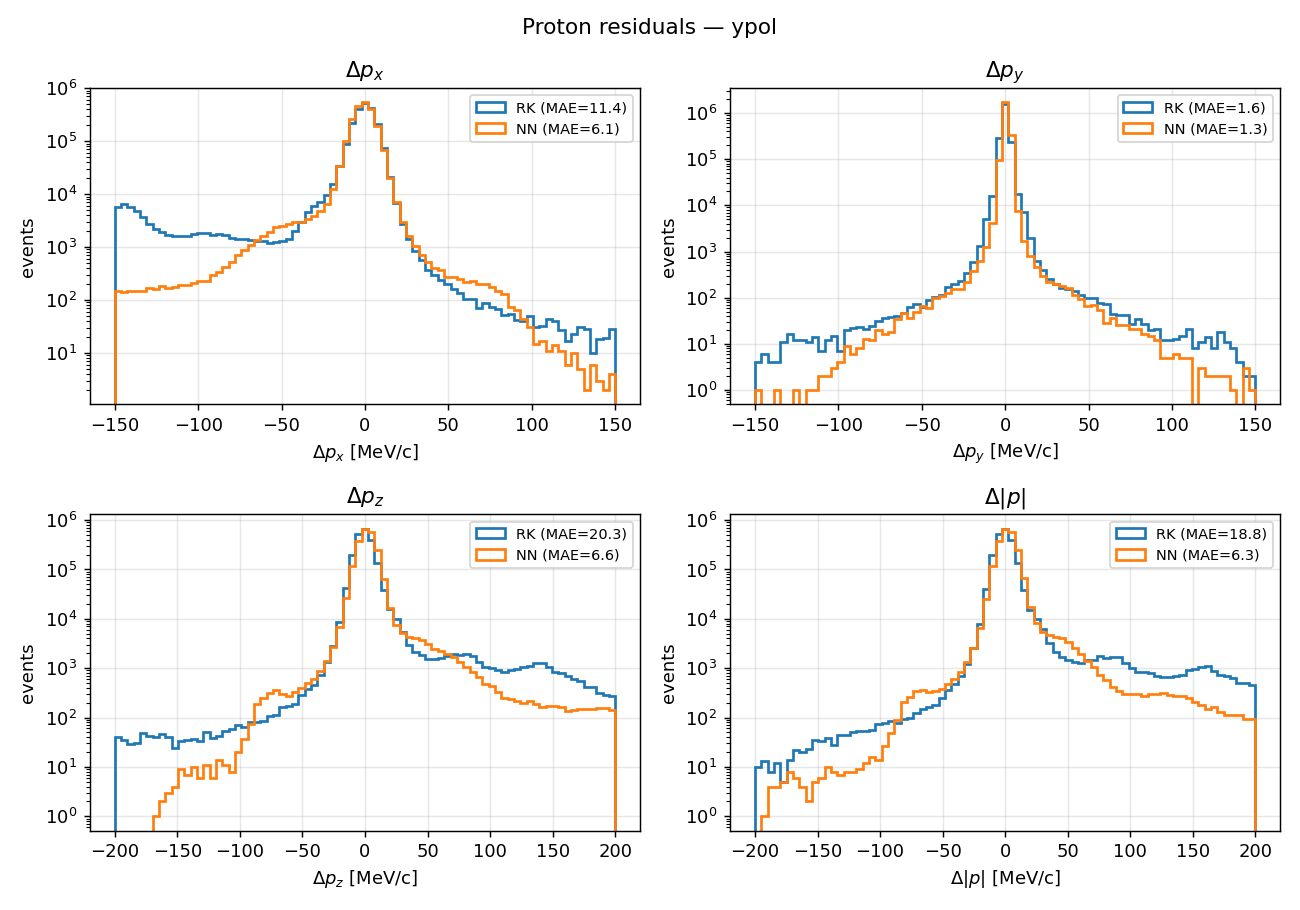
\includegraphics[width=0.95\textwidth]{figures/rk_vs_nn_breakup/proton_residuals_ypol.png}
\caption{Proton residual distributions, ypol.}
\end{figure}

\begin{figure}[h]\centering
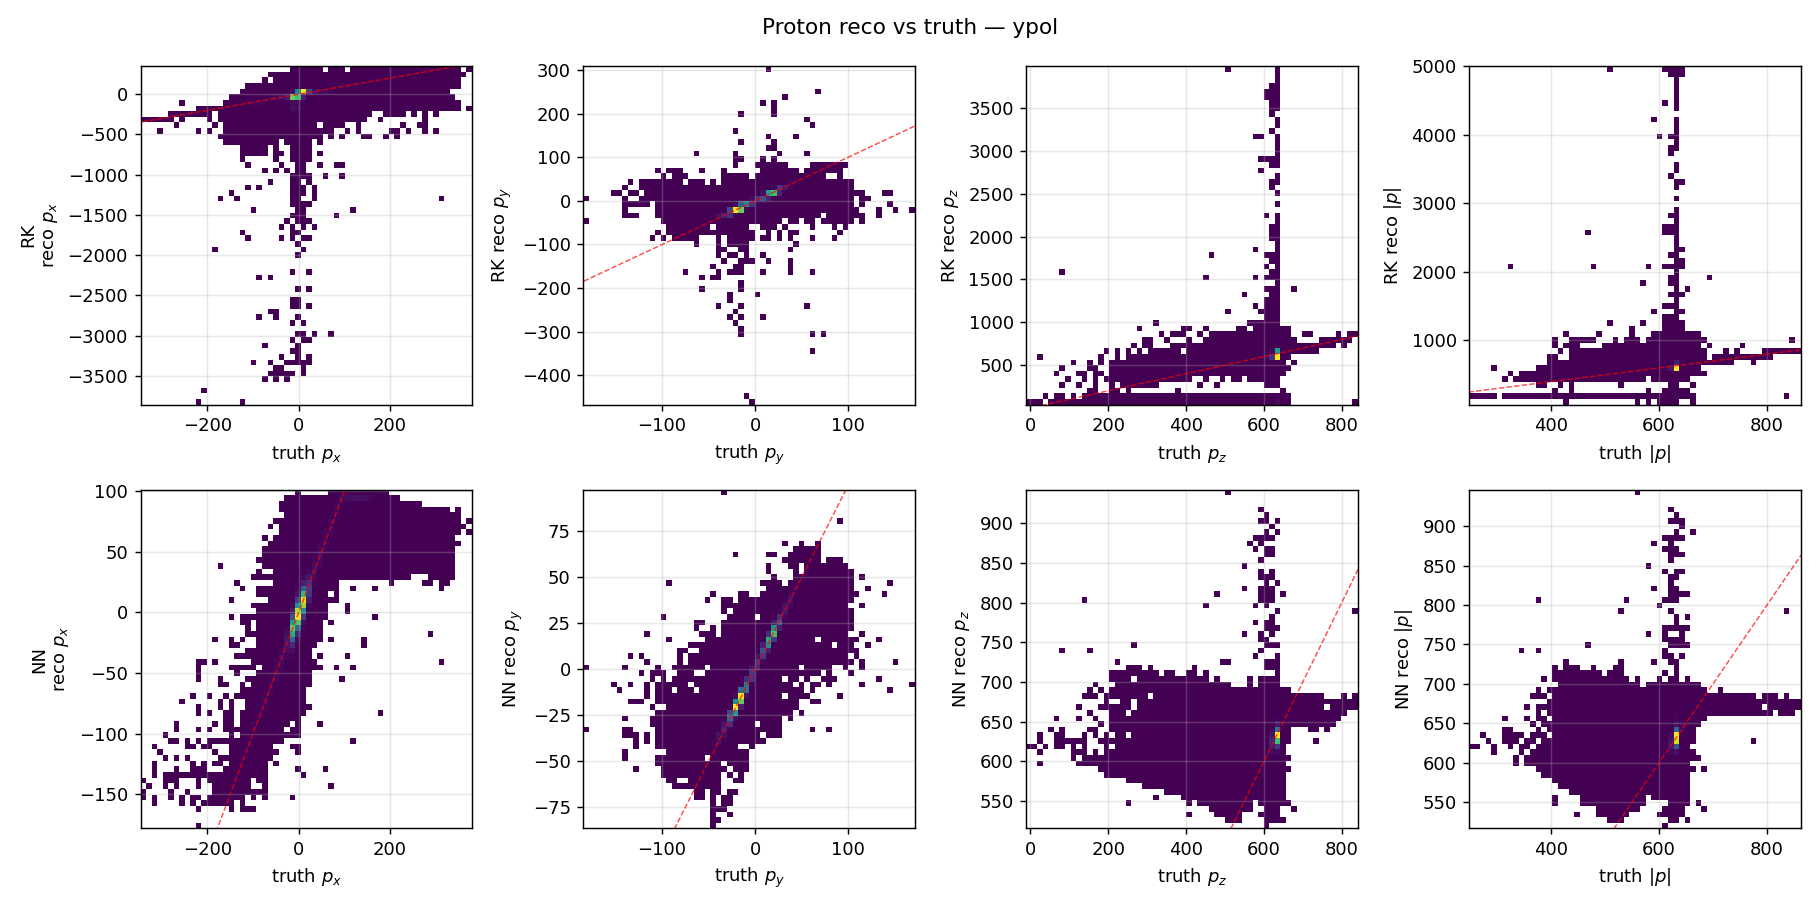
\includegraphics[width=0.95\textwidth]{figures/rk_vs_nn_breakup/proton_reco_vs_truth_ypol.png}
\caption{Proton reco vs truth 2D scatter, ypol.}
\end{figure}

\begin{figure}[h]\centering
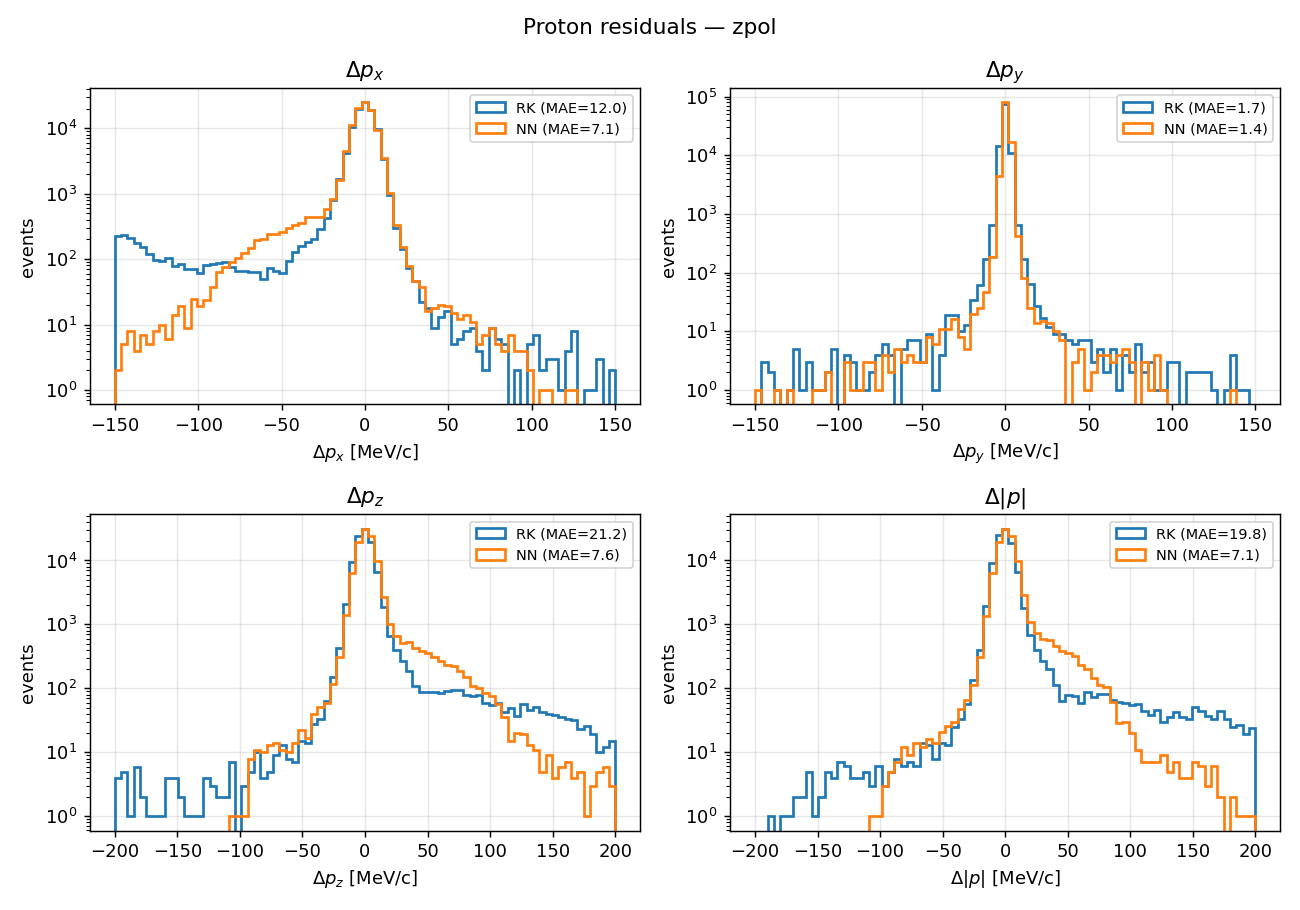
\includegraphics[width=0.95\textwidth]{figures/rk_vs_nn_breakup/proton_residuals_zpol.png}
\caption{Proton residual distributions, zpol.}
\end{figure}

\begin{figure}[h]\centering
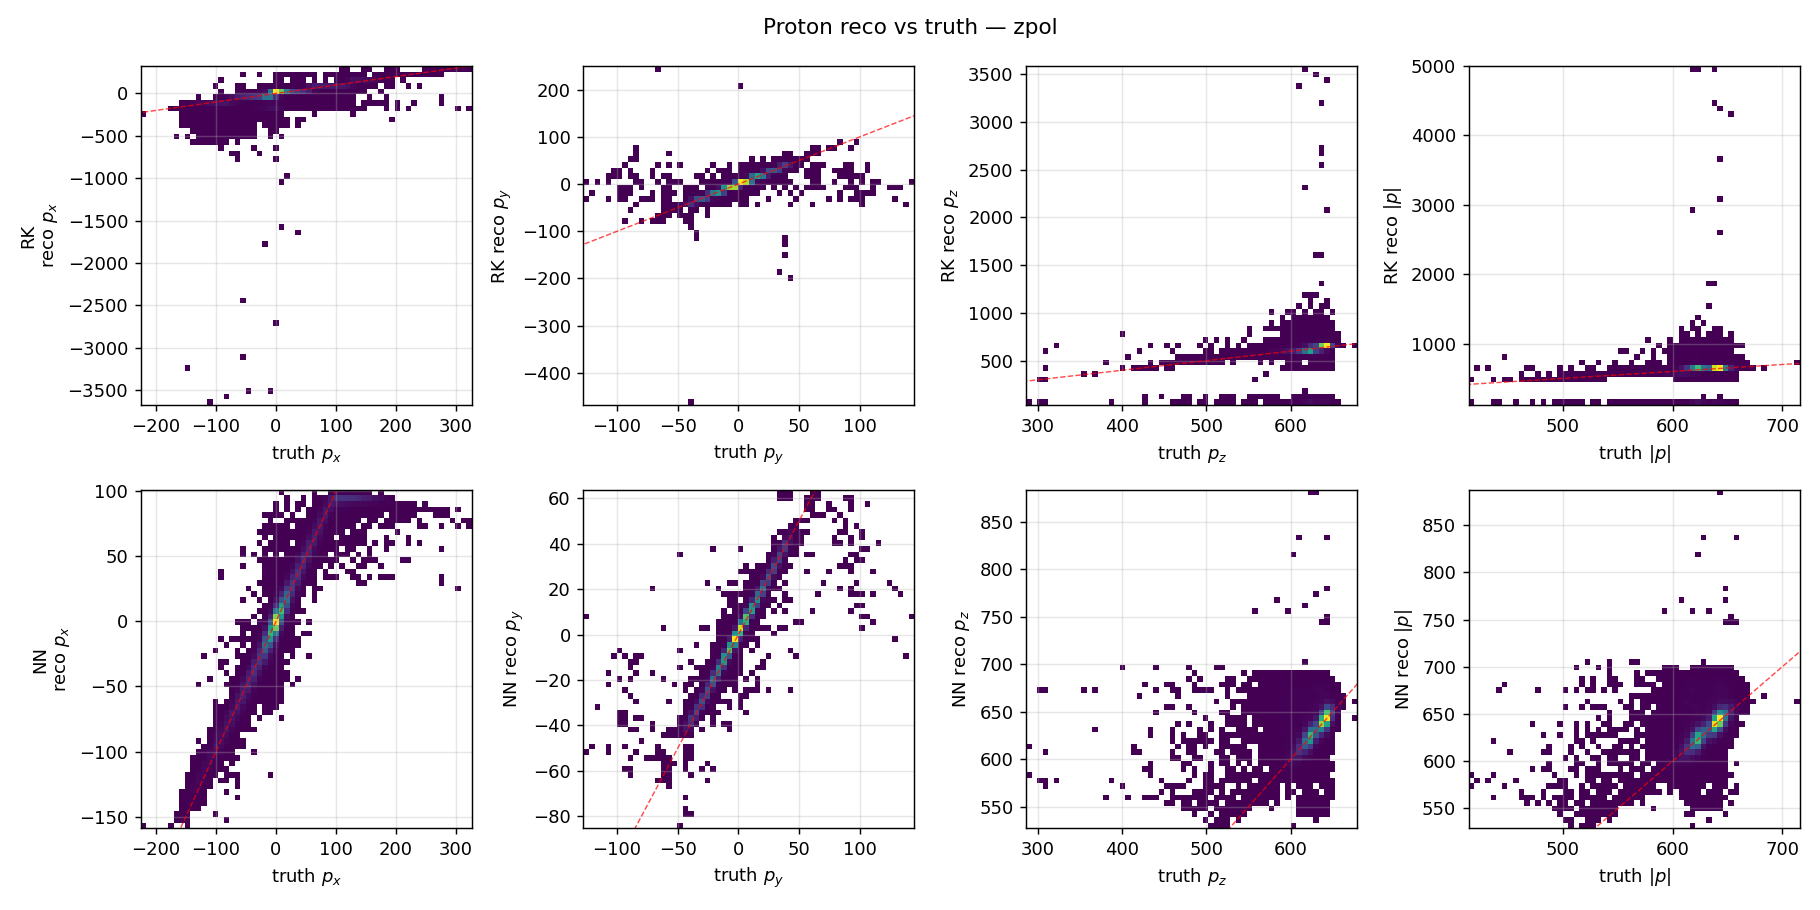
\includegraphics[width=0.95\textwidth]{figures/rk_vs_nn_breakup/proton_reco_vs_truth_zpol.png}
\caption{Proton reco vs truth 2D scatter, zpol.}
\end{figure}

\subsection{Per-event agreement (RK vs NN)}
For each event, compare $|p_{RK}-p_{truth}|$ vs $|p_{NN}-p_{truth}|$. Points below the $y=x$ line are events where RK is closer to truth; above means NN is closer.

\begin{figure}[h]\centering
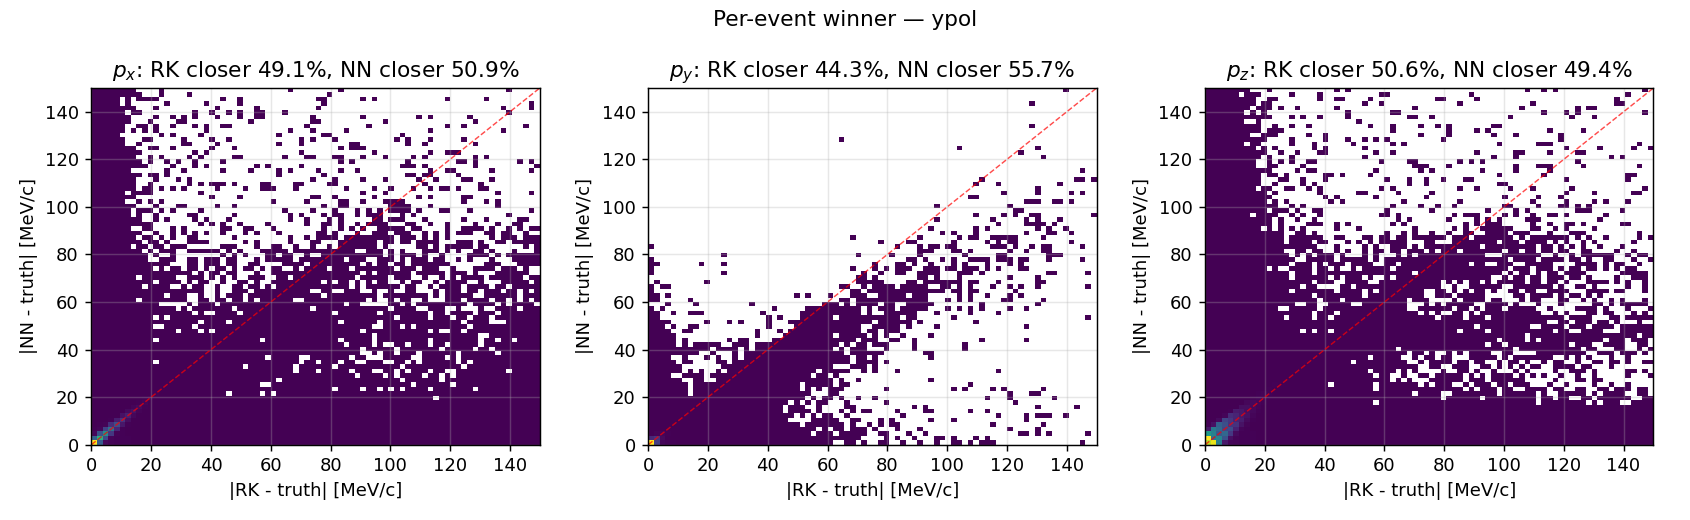
\includegraphics[width=0.95\textwidth]{figures/rk_vs_nn_breakup/proton_per_event_winner_ypol.png}
\caption{Per-event winner, ypol.}
\end{figure}

\begin{figure}[h]\centering
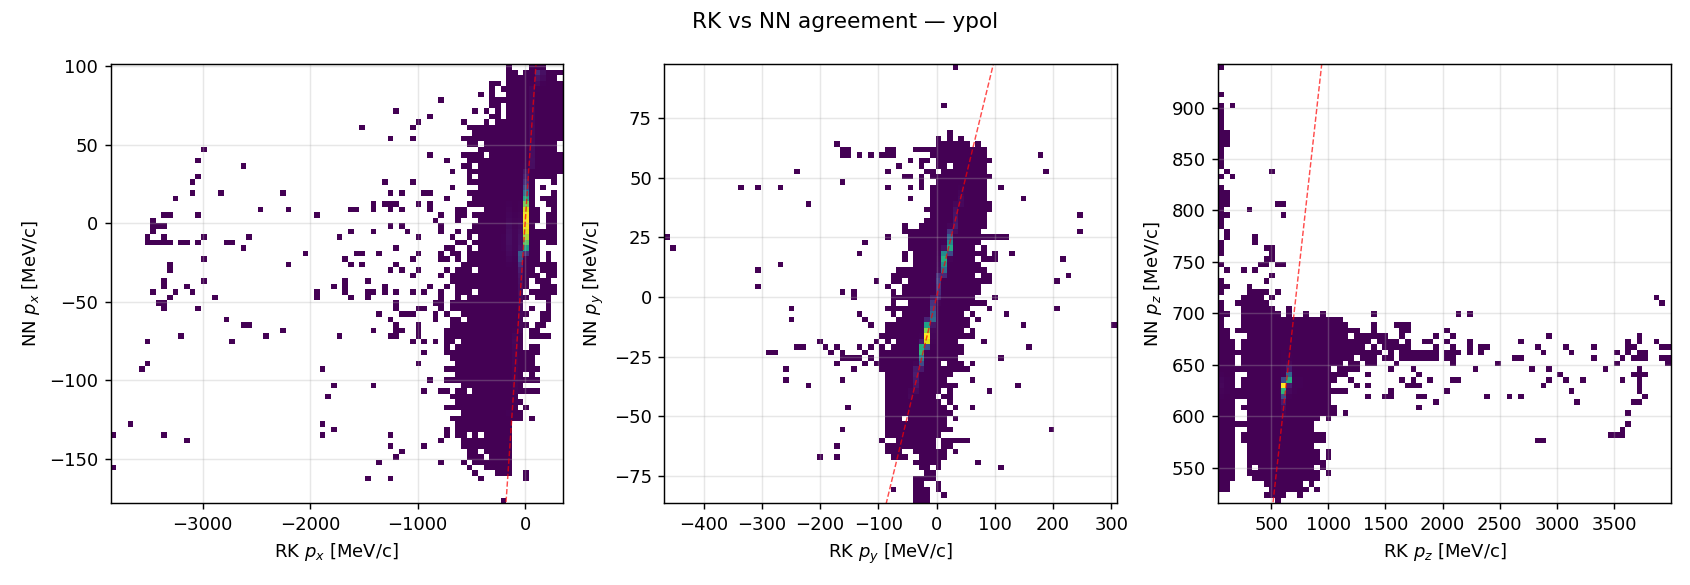
\includegraphics[width=0.95\textwidth]{figures/rk_vs_nn_breakup/proton_rk_vs_nn_agreement_ypol.png}
\caption{RK vs NN direct agreement, ypol.}
\end{figure}

\begin{figure}[h]\centering
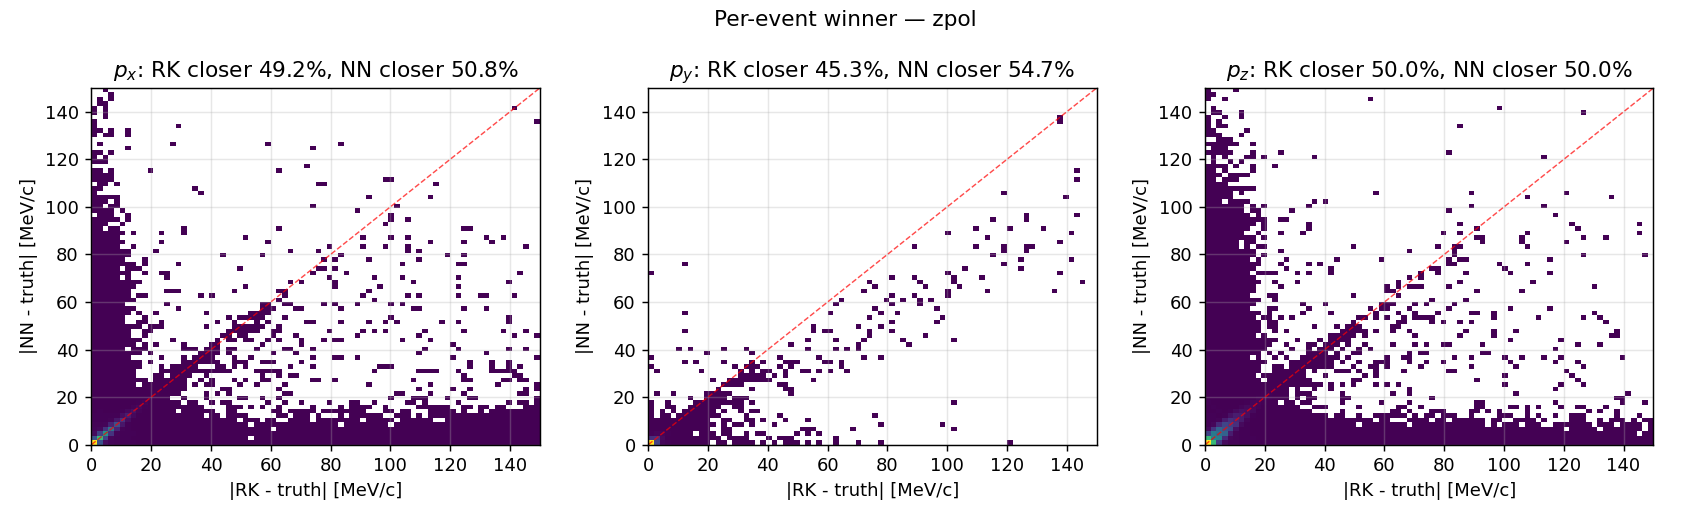
\includegraphics[width=0.95\textwidth]{figures/rk_vs_nn_breakup/proton_per_event_winner_zpol.png}
\caption{Per-event winner, zpol.}
\end{figure}

\begin{figure}[h]\centering
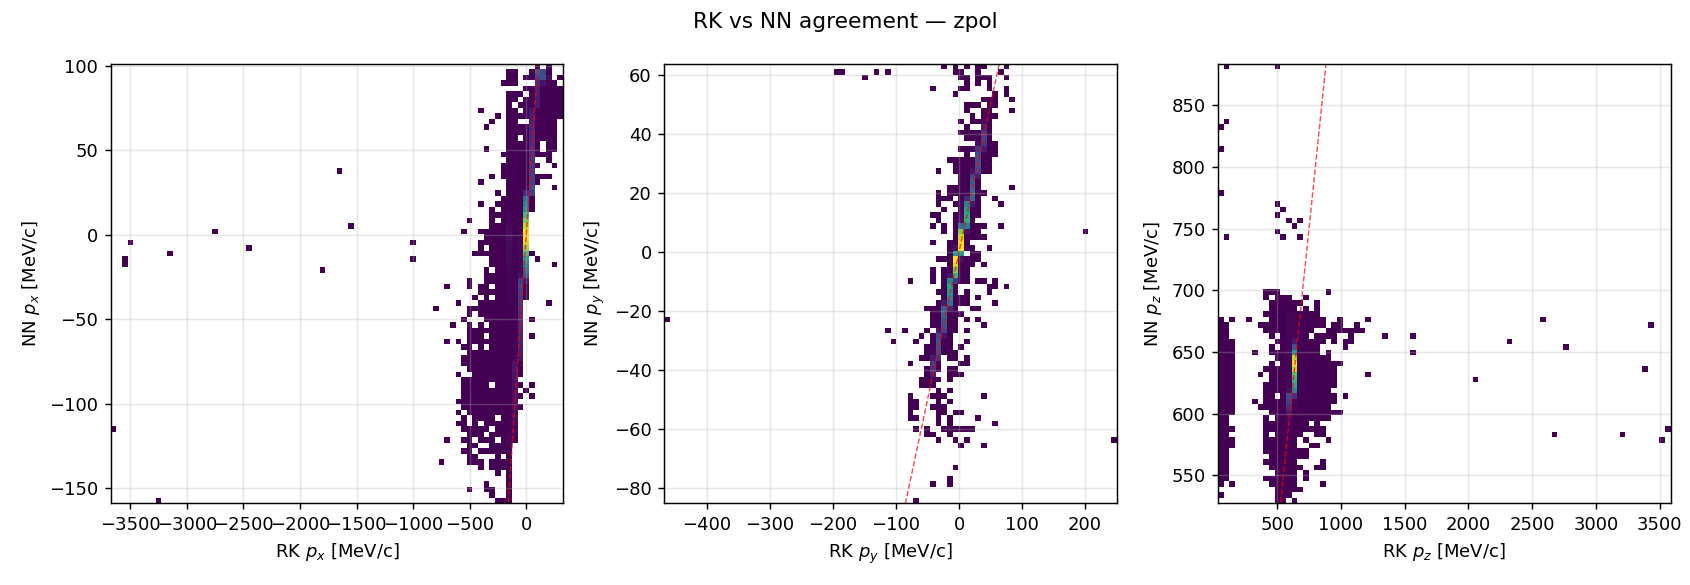
\includegraphics[width=0.95\textwidth]{figures/rk_vs_nn_breakup/proton_rk_vs_nn_agreement_zpol.png}
\caption{RK vs NN direct agreement, zpol.}
\end{figure}

\subsection{Per-cell breakdown}
\begin{figure}[h]\centering
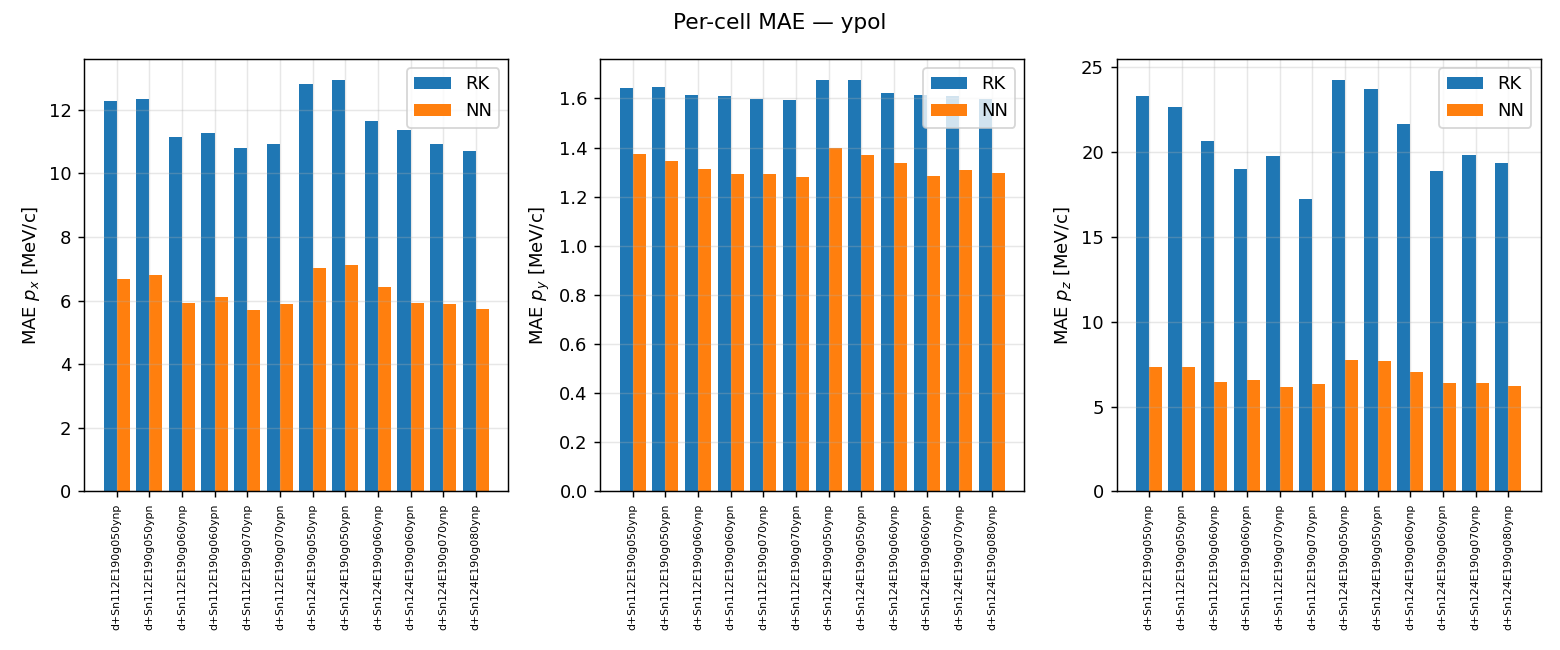
\includegraphics[width=0.95\textwidth]{figures/rk_vs_nn_breakup/proton_per_cell_mae_ypol.png}
\caption{Per-cell MAE, ypol.}
\end{figure}

\begin{figure}[h]\centering
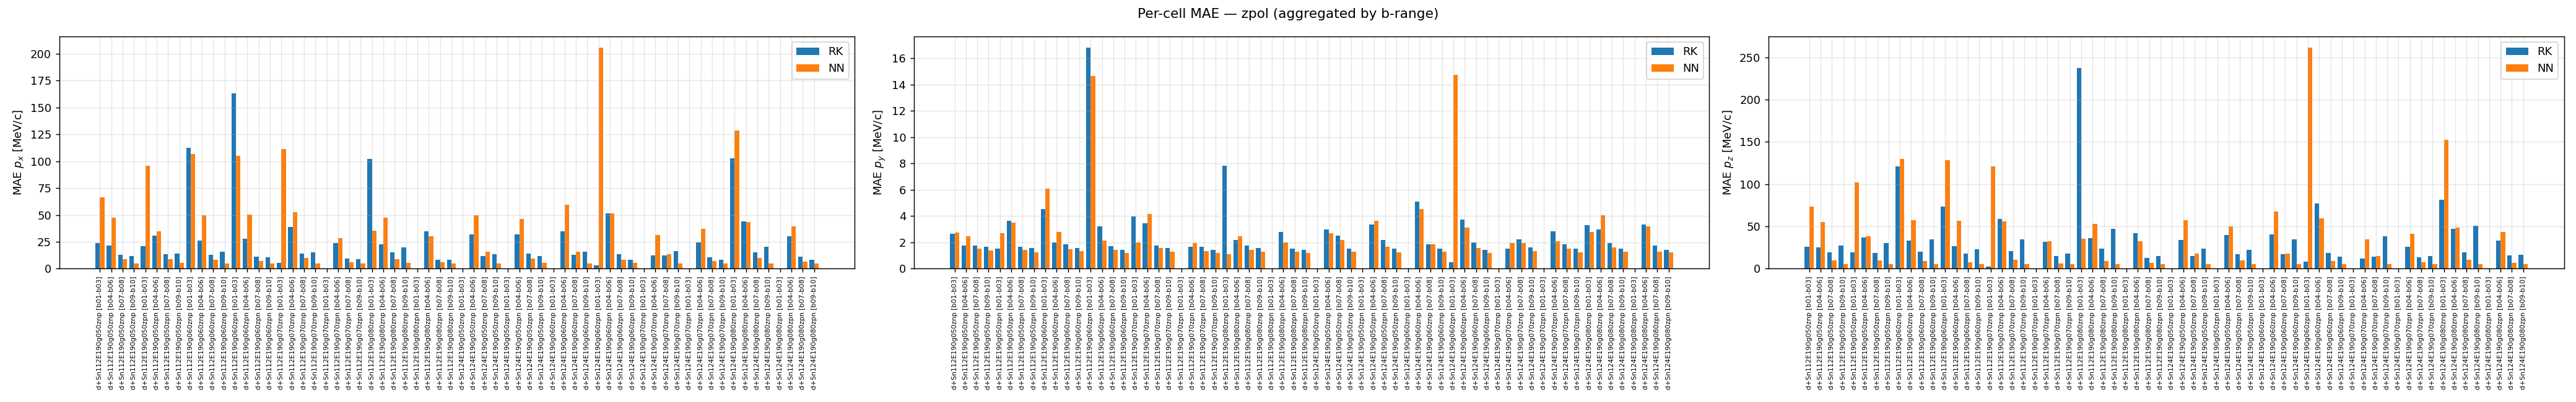
\includegraphics[width=0.95\textwidth]{figures/rk_vs_nn_breakup/proton_per_cell_mae_zpol.png}
\caption{Per-cell MAE, zpol (aggregated by b-range).}
\end{figure}

\begin{figure}[h]\centering
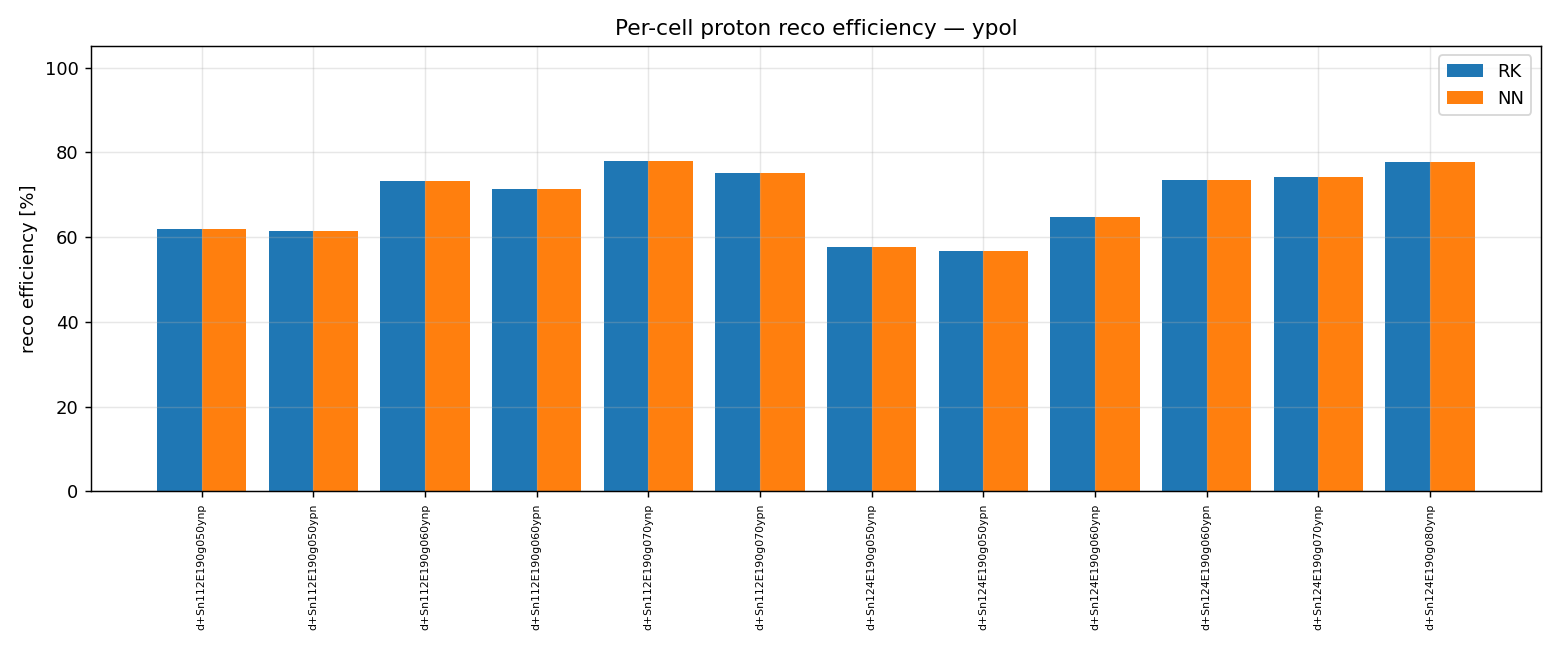
\includegraphics[width=0.95\textwidth]{figures/rk_vs_nn_breakup/proton_efficiency_per_cell_ypol.png}
\caption{Per-cell proton reco efficiency, ypol.}
\end{figure}

\begin{figure}[h]\centering
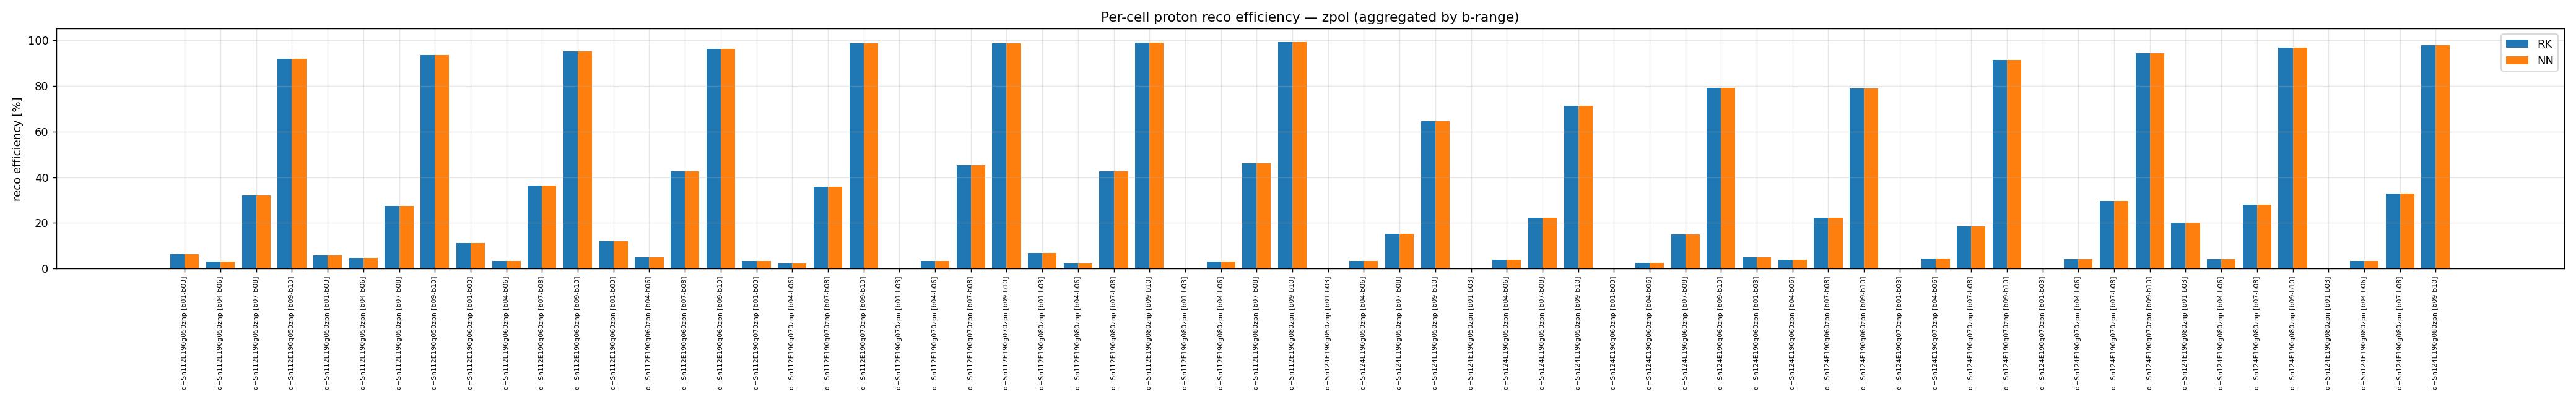
\includegraphics[width=0.95\textwidth]{figures/rk_vs_nn_breakup/proton_efficiency_per_cell_zpol.png}
\caption{Per-cell proton reco efficiency, zpol (aggregated by b-range).}
\end{figure}

\subsection{RK uncertainty calibration (pull)}
Pull $= (|p|_{RK} - |p|_{truth}) / \sigma_p$. Should be $\sim\mathcal{N}(0,1)$ if Fisher uncertainties are calibrated.

\begin{figure}[h]\centering
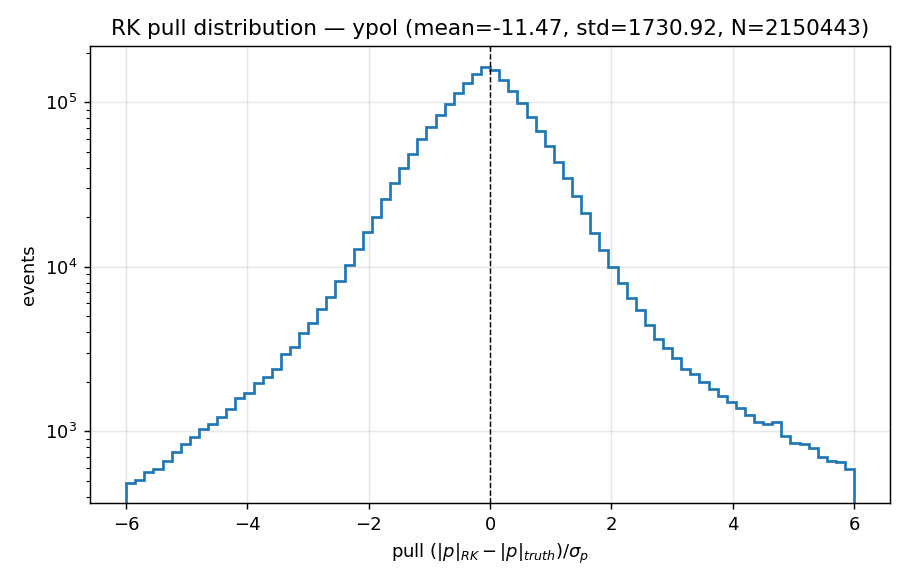
\includegraphics[width=0.7\textwidth]{figures/rk_vs_nn_breakup/proton_rk_pull_ypol.png}
\caption{RK pull distribution, ypol.}
\end{figure}

\begin{figure}[h]\centering
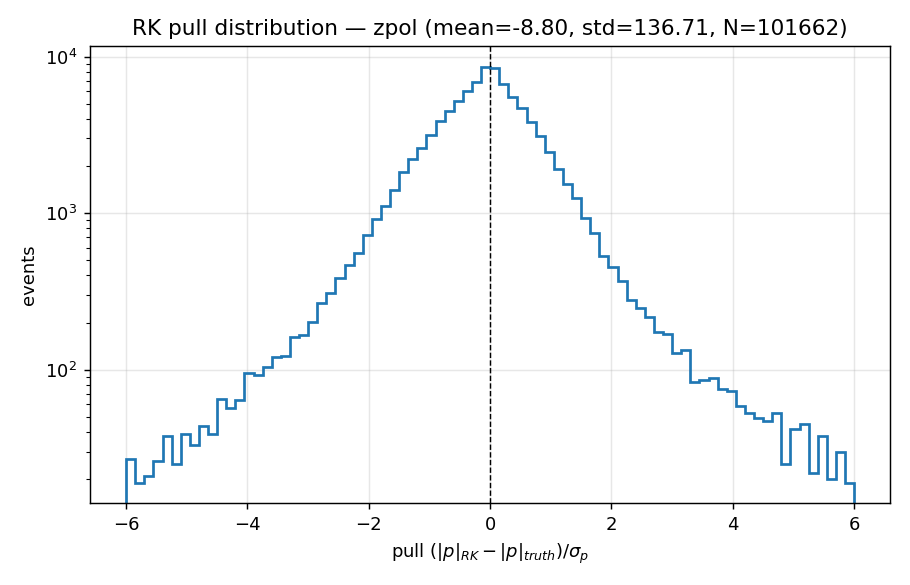
\includegraphics[width=0.7\textwidth]{figures/rk_vs_nn_breakup/proton_rk_pull_zpol.png}
\caption{RK pull distribution, zpol.}
\end{figure}

\section{Neutron reconstruction --- truth vs reco}
Neutron momentum is reconstructed by the NEBULA $\beta$-method in both RK and NN backends (the backend choice only affects proton reconstruction). Residuals below are therefore single-backend (NN file used).

\begin{figure}[h]\centering
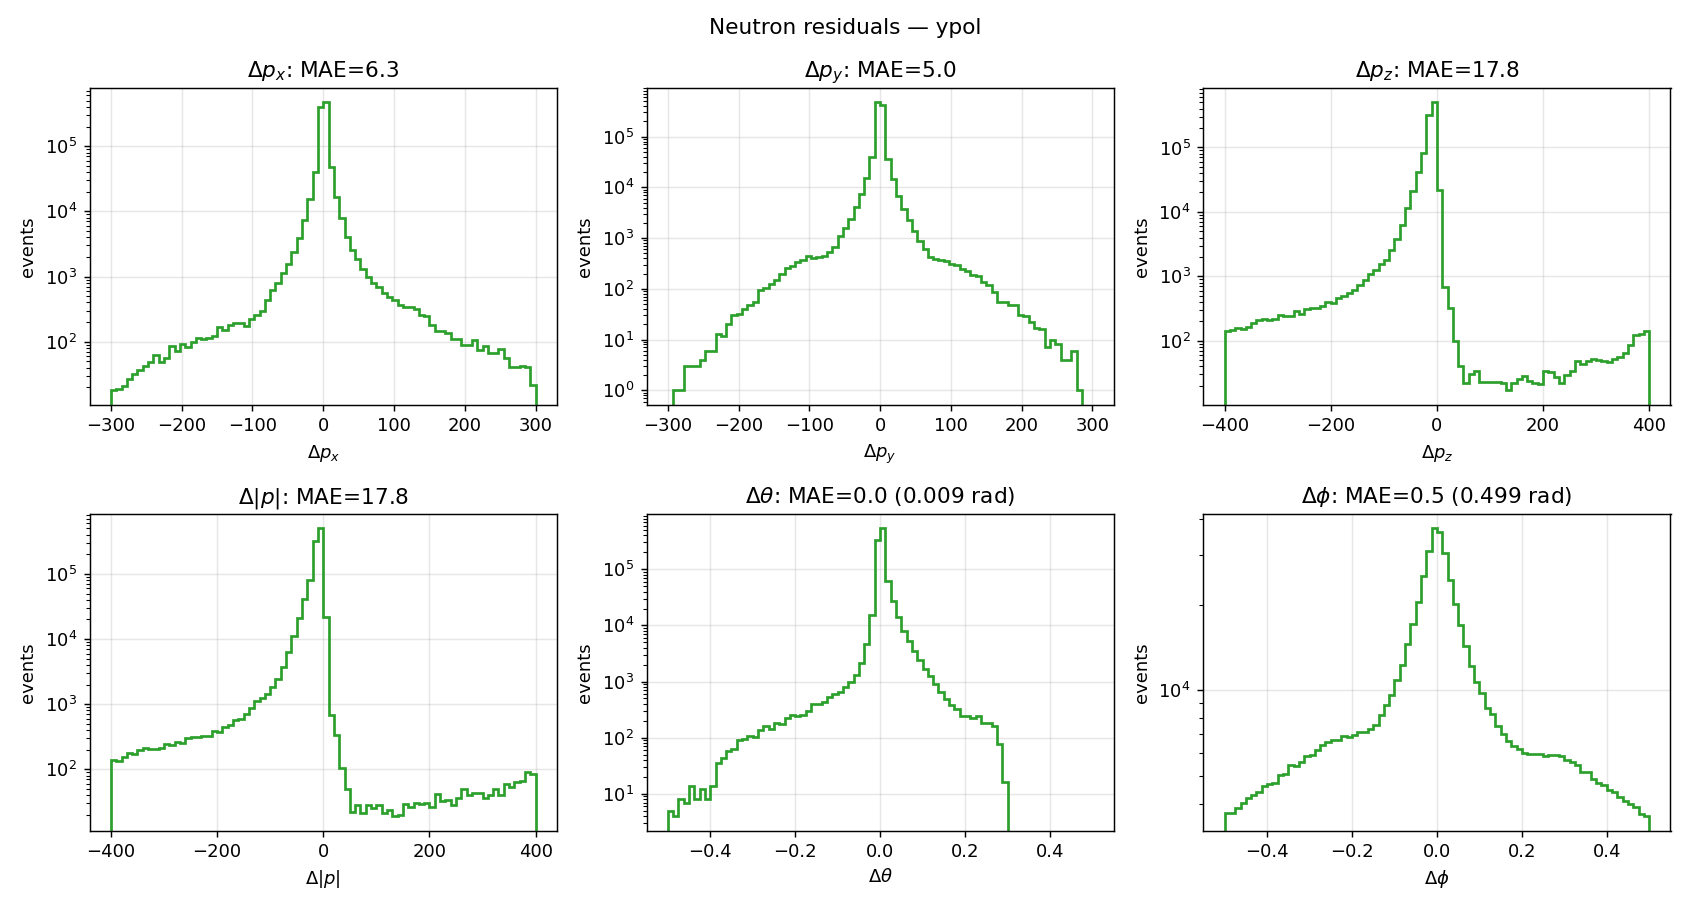
\includegraphics[width=0.95\textwidth]{figures/rk_vs_nn_breakup/neutron_residuals_ypol.png}
\caption{Neutron residual distributions, ypol.}
\end{figure}

\begin{figure}[h]\centering
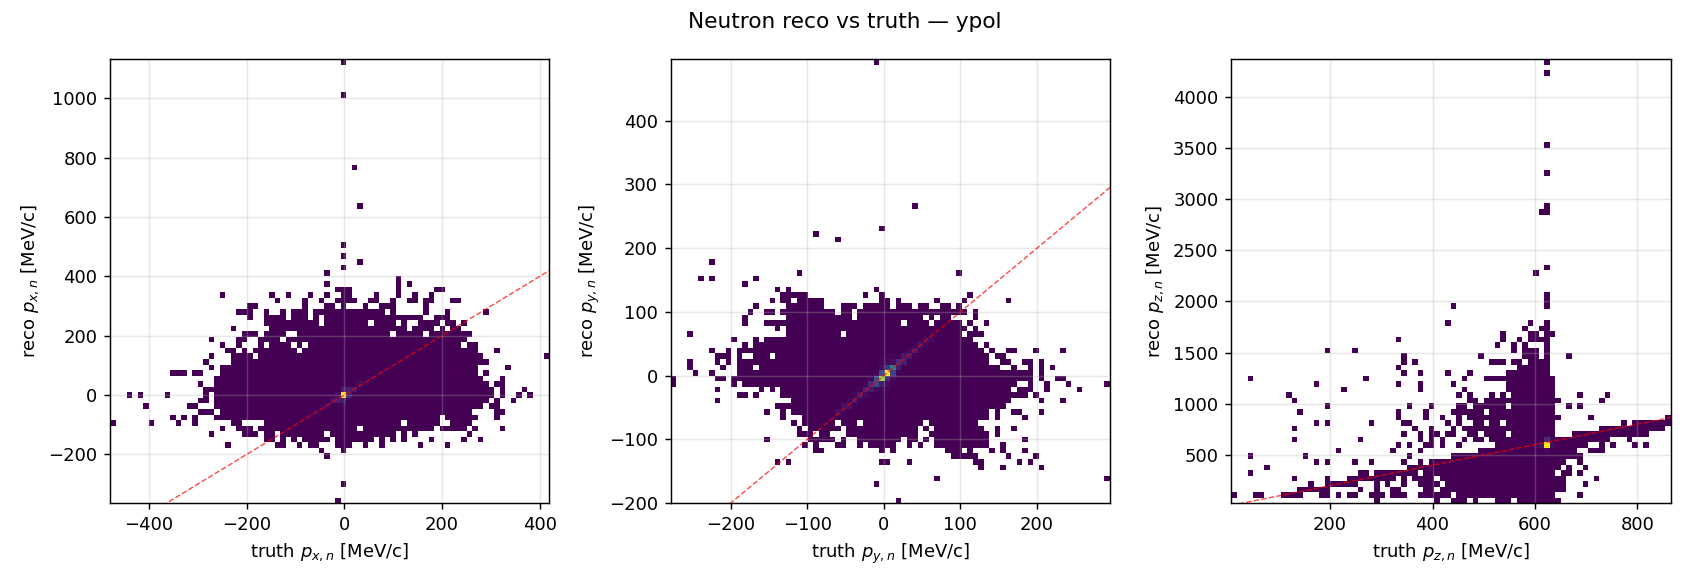
\includegraphics[width=0.95\textwidth]{figures/rk_vs_nn_breakup/neutron_reco_vs_truth_ypol.png}
\caption{Neutron reco vs truth 2D scatter, ypol.}
\end{figure}

\begin{figure}[h]\centering
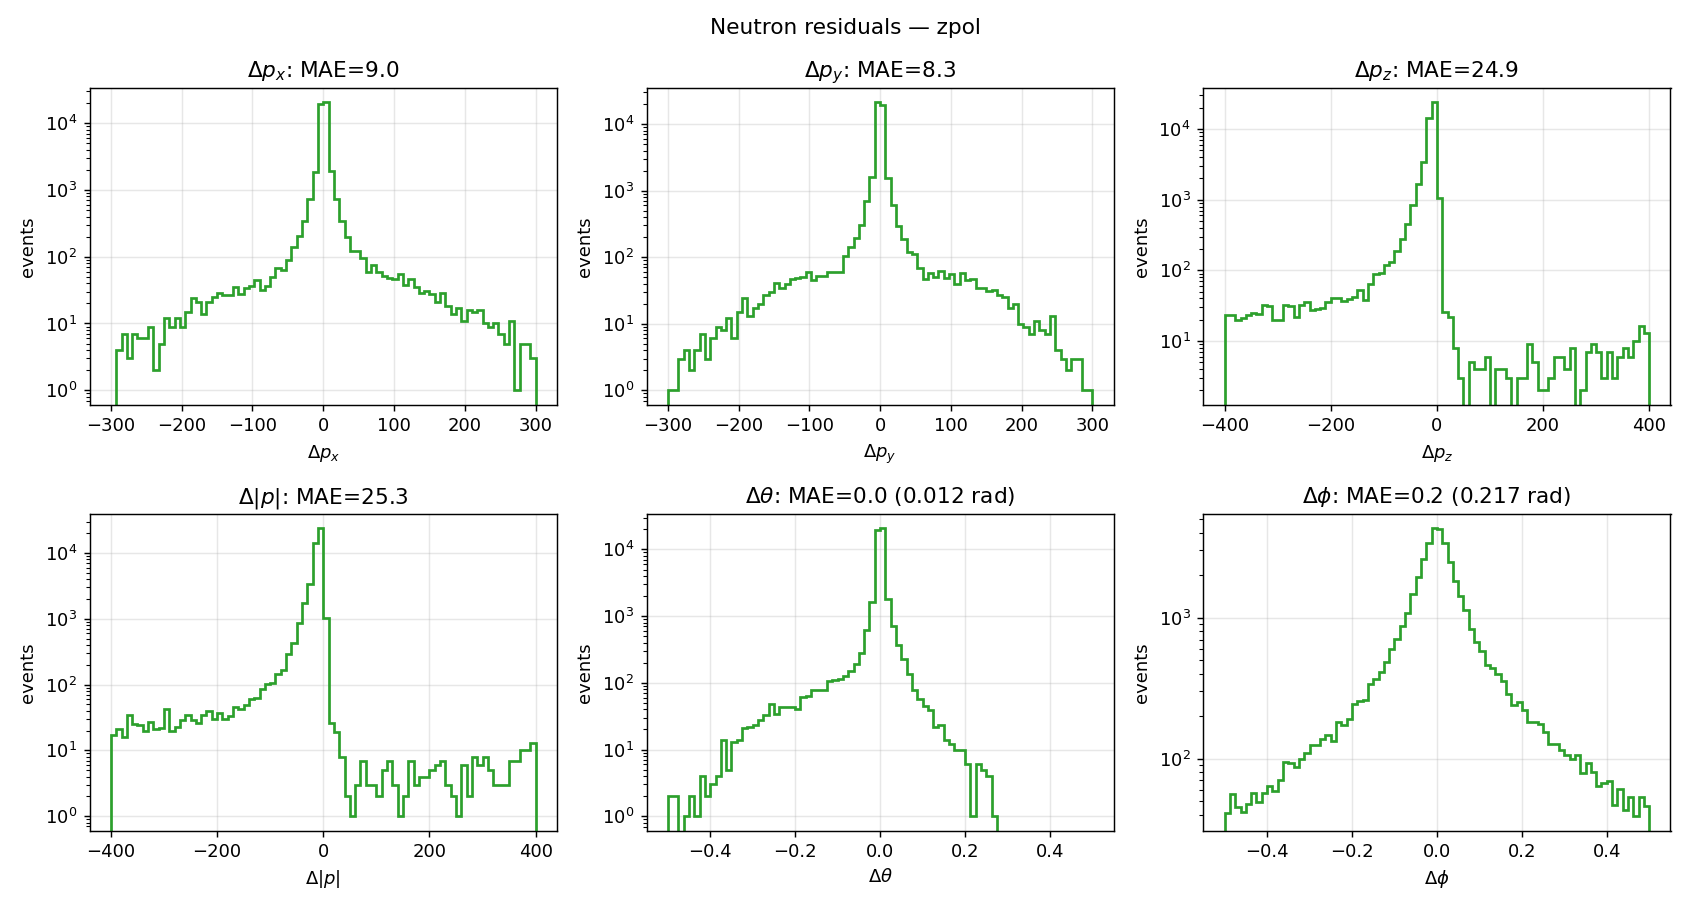
\includegraphics[width=0.95\textwidth]{figures/rk_vs_nn_breakup/neutron_residuals_zpol.png}
\caption{Neutron residual distributions, zpol.}
\end{figure}

\begin{figure}[h]\centering
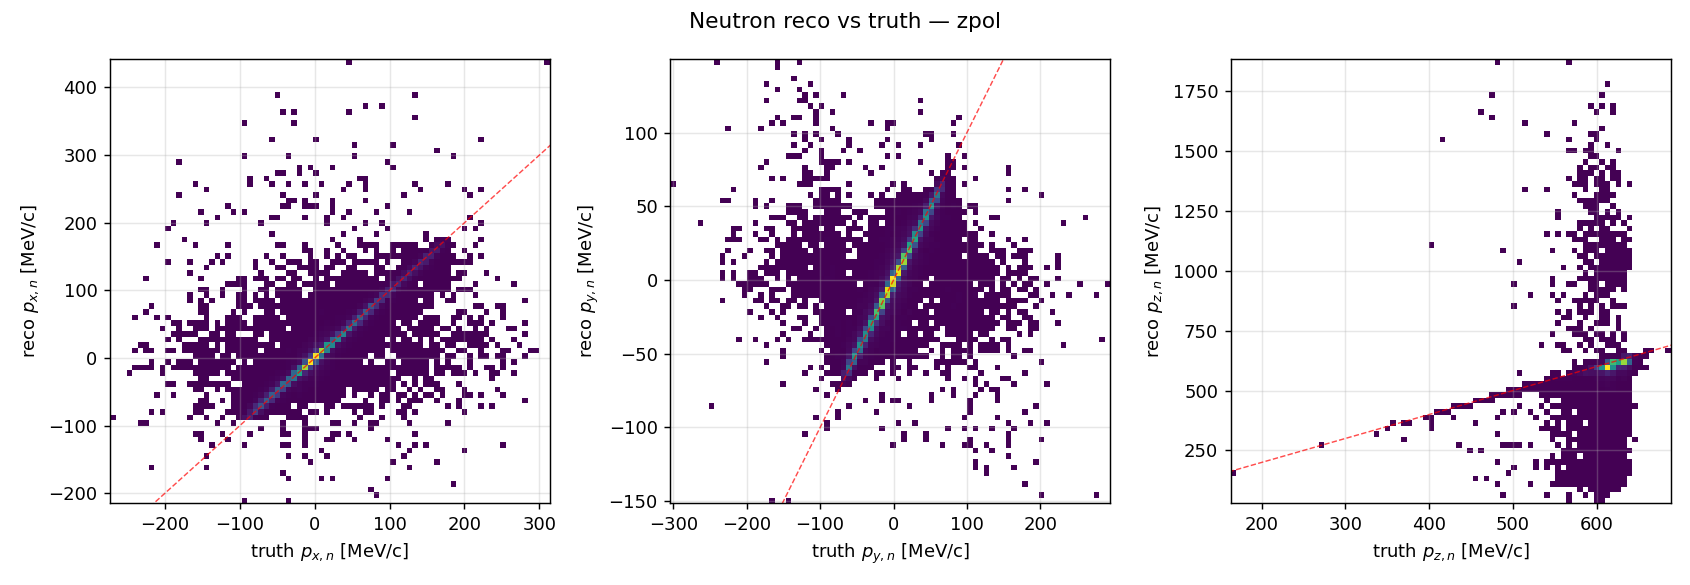
\includegraphics[width=0.95\textwidth]{figures/rk_vs_nn_breakup/neutron_reco_vs_truth_zpol.png}
\caption{Neutron reco vs truth 2D scatter, zpol.}
\end{figure}

\section{Conclusion}
(To be filled in after inspecting the figures.)

\appendix
\section{Per-cell numeric table}
(See \texttt{summary.json} for full per-cell numeric breakdown.)

\end{document}